\documentclass[]{article}
\usepackage{lmodern}
\usepackage{amssymb,amsmath}
\usepackage{ifxetex,ifluatex}
\usepackage{fixltx2e} % provides \textsubscript
\ifnum 0\ifxetex 1\fi\ifluatex 1\fi=0 % if pdftex
  \usepackage[T1]{fontenc}
  \usepackage[utf8]{inputenc}
\else % if luatex or xelatex
  \ifxetex
    \usepackage{mathspec}
  \else
    \usepackage{fontspec}
  \fi
  \defaultfontfeatures{Ligatures=TeX,Scale=MatchLowercase}
\fi
% use upquote if available, for straight quotes in verbatim environments
\IfFileExists{upquote.sty}{\usepackage{upquote}}{}
% use microtype if available
\IfFileExists{microtype.sty}{%
\usepackage{microtype}
\UseMicrotypeSet[protrusion]{basicmath} % disable protrusion for tt fonts
}{}
\usepackage[margin=1in]{geometry}
\usepackage{hyperref}
\hypersetup{unicode=true,
            pdftitle={Generalized Linear Models},
            pdfauthor={Robert Edwards},
            pdfborder={0 0 0},
            breaklinks=true}
\urlstyle{same}  % don't use monospace font for urls
\usepackage{color}
\usepackage{fancyvrb}
\newcommand{\VerbBar}{|}
\newcommand{\VERB}{\Verb[commandchars=\\\{\}]}
\DefineVerbatimEnvironment{Highlighting}{Verbatim}{commandchars=\\\{\}}
% Add ',fontsize=\small' for more characters per line
\usepackage{framed}
\definecolor{shadecolor}{RGB}{248,248,248}
\newenvironment{Shaded}{\begin{snugshade}}{\end{snugshade}}
\newcommand{\KeywordTok}[1]{\textcolor[rgb]{0.13,0.29,0.53}{\textbf{#1}}}
\newcommand{\DataTypeTok}[1]{\textcolor[rgb]{0.13,0.29,0.53}{#1}}
\newcommand{\DecValTok}[1]{\textcolor[rgb]{0.00,0.00,0.81}{#1}}
\newcommand{\BaseNTok}[1]{\textcolor[rgb]{0.00,0.00,0.81}{#1}}
\newcommand{\FloatTok}[1]{\textcolor[rgb]{0.00,0.00,0.81}{#1}}
\newcommand{\ConstantTok}[1]{\textcolor[rgb]{0.00,0.00,0.00}{#1}}
\newcommand{\CharTok}[1]{\textcolor[rgb]{0.31,0.60,0.02}{#1}}
\newcommand{\SpecialCharTok}[1]{\textcolor[rgb]{0.00,0.00,0.00}{#1}}
\newcommand{\StringTok}[1]{\textcolor[rgb]{0.31,0.60,0.02}{#1}}
\newcommand{\VerbatimStringTok}[1]{\textcolor[rgb]{0.31,0.60,0.02}{#1}}
\newcommand{\SpecialStringTok}[1]{\textcolor[rgb]{0.31,0.60,0.02}{#1}}
\newcommand{\ImportTok}[1]{#1}
\newcommand{\CommentTok}[1]{\textcolor[rgb]{0.56,0.35,0.01}{\textit{#1}}}
\newcommand{\DocumentationTok}[1]{\textcolor[rgb]{0.56,0.35,0.01}{\textbf{\textit{#1}}}}
\newcommand{\AnnotationTok}[1]{\textcolor[rgb]{0.56,0.35,0.01}{\textbf{\textit{#1}}}}
\newcommand{\CommentVarTok}[1]{\textcolor[rgb]{0.56,0.35,0.01}{\textbf{\textit{#1}}}}
\newcommand{\OtherTok}[1]{\textcolor[rgb]{0.56,0.35,0.01}{#1}}
\newcommand{\FunctionTok}[1]{\textcolor[rgb]{0.00,0.00,0.00}{#1}}
\newcommand{\VariableTok}[1]{\textcolor[rgb]{0.00,0.00,0.00}{#1}}
\newcommand{\ControlFlowTok}[1]{\textcolor[rgb]{0.13,0.29,0.53}{\textbf{#1}}}
\newcommand{\OperatorTok}[1]{\textcolor[rgb]{0.81,0.36,0.00}{\textbf{#1}}}
\newcommand{\BuiltInTok}[1]{#1}
\newcommand{\ExtensionTok}[1]{#1}
\newcommand{\PreprocessorTok}[1]{\textcolor[rgb]{0.56,0.35,0.01}{\textit{#1}}}
\newcommand{\AttributeTok}[1]{\textcolor[rgb]{0.77,0.63,0.00}{#1}}
\newcommand{\RegionMarkerTok}[1]{#1}
\newcommand{\InformationTok}[1]{\textcolor[rgb]{0.56,0.35,0.01}{\textbf{\textit{#1}}}}
\newcommand{\WarningTok}[1]{\textcolor[rgb]{0.56,0.35,0.01}{\textbf{\textit{#1}}}}
\newcommand{\AlertTok}[1]{\textcolor[rgb]{0.94,0.16,0.16}{#1}}
\newcommand{\ErrorTok}[1]{\textcolor[rgb]{0.64,0.00,0.00}{\textbf{#1}}}
\newcommand{\NormalTok}[1]{#1}
\usepackage{longtable,booktabs}
\usepackage{graphicx,grffile}
\makeatletter
\def\maxwidth{\ifdim\Gin@nat@width>\linewidth\linewidth\else\Gin@nat@width\fi}
\def\maxheight{\ifdim\Gin@nat@height>\textheight\textheight\else\Gin@nat@height\fi}
\makeatother
% Scale images if necessary, so that they will not overflow the page
% margins by default, and it is still possible to overwrite the defaults
% using explicit options in \includegraphics[width, height, ...]{}
\setkeys{Gin}{width=\maxwidth,height=\maxheight,keepaspectratio}
\IfFileExists{parskip.sty}{%
\usepackage{parskip}
}{% else
\setlength{\parindent}{0pt}
\setlength{\parskip}{6pt plus 2pt minus 1pt}
}
\setlength{\emergencystretch}{3em}  % prevent overfull lines
\providecommand{\tightlist}{%
  \setlength{\itemsep}{0pt}\setlength{\parskip}{0pt}}
\setcounter{secnumdepth}{5}
% Redefines (sub)paragraphs to behave more like sections
\ifx\paragraph\undefined\else
\let\oldparagraph\paragraph
\renewcommand{\paragraph}[1]{\oldparagraph{#1}\mbox{}}
\fi
\ifx\subparagraph\undefined\else
\let\oldsubparagraph\subparagraph
\renewcommand{\subparagraph}[1]{\oldsubparagraph{#1}\mbox{}}
\fi

%%% Use protect on footnotes to avoid problems with footnotes in titles
\let\rmarkdownfootnote\footnote%
\def\footnote{\protect\rmarkdownfootnote}

%%% Change title format to be more compact
\usepackage{titling}

% Create subtitle command for use in maketitle
\newcommand{\subtitle}[1]{
  \posttitle{
    \begin{center}\large#1\end{center}
    }
}

\setlength{\droptitle}{-2em}
  \title{Generalized Linear Models}
  \pretitle{\vspace{\droptitle}\centering\huge}
  \posttitle{\par}
  \author{Robert Edwards}
  \preauthor{\centering\large\emph}
  \postauthor{\par}
  \predate{\centering\large\emph}
  \postdate{\par}
  \date{8 March 2019}

\usepackage{booktabs}
\usepackage{longtable}
\usepackage{array}
\usepackage{multirow}
\usepackage[table]{xcolor}
\usepackage{wrapfig}
\usepackage{float}
\usepackage{colortbl}
\usepackage{pdflscape}
\usepackage{tabu}
\usepackage{threeparttable}
\usepackage[normalem]{ulem}

\usepackage{float} \floatplacement{figure}{H}

\begin{document}
\maketitle

\section{Introduction}\label{sec:Intro}

In Weeks 3 and 6 we looked at modelling data using linear regression
models where we had:

\begin{itemize}
\tightlist
\item
  a \textbf{continuous response variable \(y\)} and
\item
  one or more \textbf{explanatory variables} \(x_1, x_2, \dots ,x_p\)
  which were \textbf{numerical} and/or \textbf{categorical} variables.
\end{itemize}

Recall that for data \((y_i,x_i), i=1, \dots, n\), where \(y\) is a
continuous response variable, we can write a simple linear regression
model as follows:
\[y_i = \alpha + \beta x_i + \epsilon_i, ~~~ \epsilon_i \sim N(0, \sigma^2)\]

where,

\begin{itemize}
\tightlist
\item
  \(y_i\) is the \(i^{th}\) observation of the continuous response
  variable;
\item
  \(\alpha\) is the \textbf{intercept} of the regression line;
\item
  \(\beta\) is the \textbf{slope} of the regression line;
\item
  \(x_i\) is the \(i^{th}\) observations of the explanatory variable;
\item
  \(\epsilon_i\) is the \(i^{th}\) random component.
\end{itemize}

Thus, the full probability model for \(y_i\) given
\$x\_i(y\_i\textbar{}x\_i) can be written as
\[y_i|x_i \sim N(\alpha + \beta x_i, \sigma^2)\]

where the mean \(\alpha + \beta x_i\) is given by the deterministic part
of the model and the variance \(\sigma^2\) by the random part. Hence we
make the assumption that the outcomes \(y_i\) are normally distributed
with mean \(\alpha + \beta x_i\) and variance \(\sigma^2\). However,
what if our response variable \(y\) is not a continuous random variable?

\subsection{Generalized Linear Models}\label{generalized-linear-models}

The main objective this week is to introduce \textbf{Generalised Linear
Models (GLMs)}, which extend the linear model framework to response
variables that don't follow the normal distribution. GLMs can be used to
model non-normal continuous response variables, but they are most
frequently used to model binary, categorical or count data. Here we
shall focus on binary/categorical response variables. The generalised
linear model can be written as:\\
\[
\begin{aligned}
y_i             &\sim f(g(\mathbf{\mu}_i)) \\
\mathbf{\mu}_i  &= \mathbf{x}^T_i \mathbf{\beta}
\end{aligned}
\]

where the response \(y_i\) is predicted through the linear combination
\(\mathbf{\mu}_i\) of explanatory variables by the link function
\(g(\cdot)\), assuming some distribution \(f(\cdot)\) for \(y_i\), and
\(\mathbf{x}^T_i\) is the \(i^{th}\) row of the design matrix
\(\mathbf{X}\). For example, the simple linear regression model above
for a continuous response variable has the normal distribution as
\(f(\cdot)\), with corresponding link function equal to the identity
function, that is, \(g(\mathbf{\mu}_i) = \mathbf{\mu}_i\).

What if our response variable \(y\) is binary (e.g.~yes/no,
success/failure, alive/dead)? That is, the independent responses \(y_i\)
can either be:

\begin{itemize}
\tightlist
\item
  \textbf{binary}, taking the value 1 (say success, with probability
  \(p_i\)) or 0 (failure, with probability \(1-p_i\)) or
\item
  \textbf{binomial}, where \(y_i\) is the number of successes in a given
  number of trial \(n_i\), with the probability of success being \(p_i\)
  and the probability of failure being \(1-p_i\)
\end{itemize}

In both cases the distribution of \(y_i\) is assumed to be binomial, but
in the first case it is \(\mbox{Bi}(1, p_i)\) and in the second case it
is \(\mbox{Bi}(n_i, p_i)\). Hence, a binary response variable \(y_i\)
has a binomial distribution with corresponding link function
\(g(\cdot)\) equal to the \textbf{logit link} function, that is\\
\[g(p_i) = \mbox{log} \Bigg( \frac{p_i}{1-p_i} \Bigg)\]

which is also referred to as the \textbf{log-odds} (since
\(\frac{p_i}{1-p_i}\) is an odds ratio). Why is such a transformation
required when looking at a binary response variable? Well here we are
interested in modelling the probability of success \(p_i\), and as we
know probabilities must be between 0 and 1 \((p_i \in [0,1])\). So if we
want to model the probability of success using a linear model we need to
ensure that the probabilities obtained are between 0 and 1. However, if
we just use the identity link function, such that
\[p_i = \mathbf{x}^T_i \mathbf{\beta}\]\\
we would need to ensure that in some way
\(\mathbf{x}^T_i \mathbf{\beta} \in [0,1]\) that is, the linear
combination of the explanatory variables and their corresponding
regression coefficients was between 0 and 1. Hence some restrictions of
some sort would need to be put in place to ensure this was the case.
However, if we use the logit link function, such that
\[\mbox{log} \Bigg( \frac{p_i}{1-p_i} \Bigg) = \mathbf{x}^T_i \mathbf{\beta}\]

No restrictions need to be in place on our estimates of the parameter
vector \(\beta\), since the inverse of the logit link function will
always give us valid probabilities since
\[p_i = \frac{\mbox{exp}(\mathbf{x}^T_i \mathbf{\beta})}{1 + \mbox{exp}(\mathbf{x}^T_i \mathbf{\beta})}  ~~~~ \in [0,1]\]

This linear regression model with a binary response variable is referred
to as \textbf{logistic regression}. As such, when it comes to looking at
binary response variables we shall be looking at odds ratios and
probabilities of success/failure. The table below is a reminder of the
distribution and link function used for the normal model we have
previously looked at as well as the logistic regression model we shall
be examining for the rest of this week.

\begin{longtable}[]{@{}lccc@{}}
\toprule
Model & Random Component & Systematic Component & Link
Function\tabularnewline
\midrule
\endhead
Normal & \(y_i \stackrel{indep}{\sim} N(\mu_i,\sigma^2)\) &
\(\mathbf{x}^T_i \mathbf{\beta}=\beta_0+\beta_1x_i+\dots\) &
\(g(\mu_i)=\mu_i\)\tabularnewline
Logistic & \(y_i \stackrel{indep}{\sim} \mbox{Bi}(1,p_i)\) &
\(\mathbf{x}^T_i \mathbf{\beta}=\beta_0+\beta_1x_i+\dots\) &
\(g(\mu_i)=\mbox{log}\bigg(\frac{\mu_i}{1-\mu_i}\bigg)=\mbox{log}\bigg(\frac{p_i}{1-p_i}\bigg)\)\tabularnewline
\bottomrule
\end{longtable}

\newpage

\section{Binary Logistic Regression with One Numerical Explanatory
Variable}\label{binary-logistic-regression-with-one-numerical-explanatory-variable}

Here we shall begin by fitting a logistic regression model with one
numerical explanatory variable. Let's return to the \texttt{evals} data
from the \texttt{moderndive} package that we examined in Week 3.

\subsection{Teaching Evaluation
Scores}\label{teaching-evaluation-scores}

Recall from previous weeks that student feedback in higher education is
extremely important when it comes to the evaluation of teaching
techniques, materials, and improvements in teaching methods and
technologies. However, there have been studies into potential bias
factors when feedback is provided, such as the physical appearance of
the teacher; see Economics of Education Review for details. Here, we
shall return to the study of student evaluations of \(n=463\) professors
from The University of Texas at Austin.

Previously, we looked at \textbf{teaching score} as our continuous
response variable and \textbf{beauty score} as our explanatory variable.
Now we shall consider \textbf{gender} as our response variable, and
hence shall have a binary response variable (female/male). We will
examine if there is any difference in \textbf{gender} by \textbf{age} of
the teaching instructors within the \texttt{evals} data set.

First, let's start by selecting the variables of interest from the
\texttt{evals} data set:

\begin{Shaded}
\begin{Highlighting}[]
\NormalTok{evals.gender <-}\StringTok{ }\NormalTok{evals }\OperatorTok
\StringTok{  }\KeywordTok{select}\NormalTok{(gender, age)}
\end{Highlighting}
\end{Shaded}

Now, let's look at a boxplot of \texttt{age} by \texttt{gender} to get
an initial impression of the data:

\begin{Shaded}
\begin{Highlighting}[]
\KeywordTok{ggplot}\NormalTok{(}\DataTypeTok{data =}\NormalTok{ evals.gender, }\KeywordTok{aes}\NormalTok{(}\DataTypeTok{x =}\NormalTok{ gender, }\DataTypeTok{y =}\NormalTok{ age, }\DataTypeTok{fill =}\NormalTok{ gender)) }\OperatorTok{+}
\StringTok{  }\KeywordTok{geom_boxplot}\NormalTok{() }\OperatorTok{+}
\StringTok{  }\KeywordTok{labs}\NormalTok{(}\DataTypeTok{x =} \StringTok{"Gender"}\NormalTok{, }\DataTypeTok{y =} \StringTok{"Age"}\NormalTok{) }\OperatorTok{+}
\StringTok{  }\KeywordTok{theme}\NormalTok{(}\DataTypeTok{legend.position =} \StringTok{"none"}\NormalTok{)}
\end{Highlighting}
\end{Shaded}

\begin{figure}
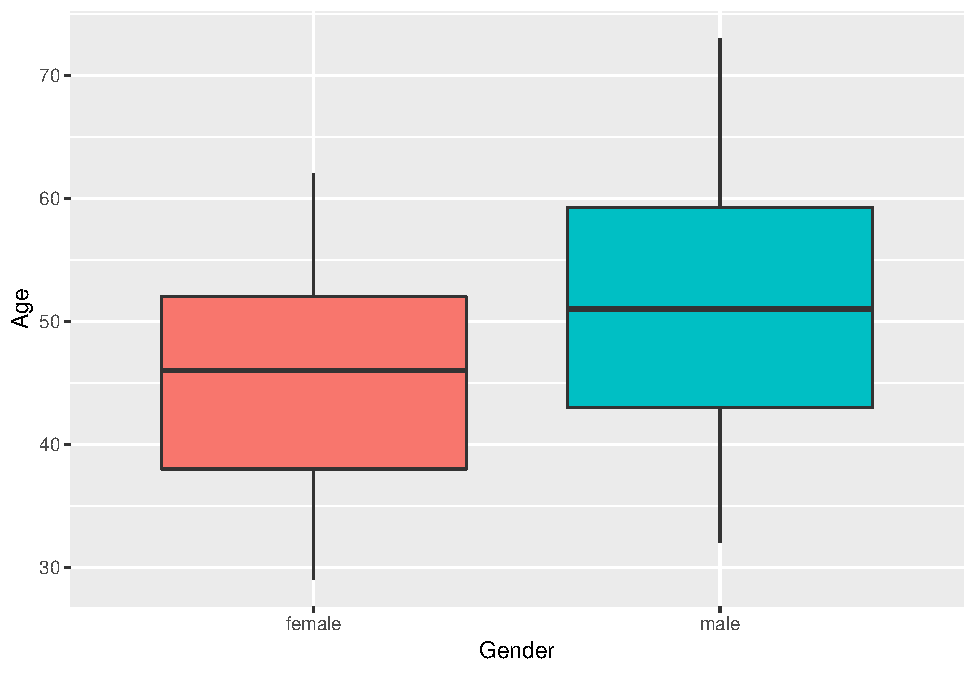
\includegraphics[width=0.5\linewidth]{DAWeek9_files/figure-latex/boxplot1-1} \caption{\label{fig.plot1}Teaching instructor age by gender}\label{fig:boxplot1}
\end{figure}

Here we can see that the male teaching instructors tend to be older than
that of their female colleagues. Now, let's fit a logistic regression
model to see whether age is a significant predictor of the odds of a
teaching instructor being male or female.

\subsection{Log-odds}\label{log-odds}

To fit a logistic regression model we will use the generalised linear
model function \texttt{glm}, which acts in a very similar manner to the
lm function we have used previously. We only have to deal with an
additional argument. The logistic regression model with gender as the
response and age as the explanatory variable is given by:


\end{document}
